\documentclass[rgb]{beamer}

\usepackage[english]{babel}
\usepackage[utf8]{inputenc}
\usepackage{xcolor}
\usepackage{listings}
\usepackage{adjustbox}
\usepackage{amsmath}
\usepackage{multirow}
\usepackage[linewidth=1pt]{mdframed}

% Graphics
\usepackage{graphicx}

\usepackage{tikz}
\usetikzlibrary{calc,shapes.multipart,chains,arrows}

% Font
\usepackage{paratype}
\setbeamerfont{frametitle}{family=\bf}

% Beamer theme settings
\usecolortheme{seagull}
\setbeamertemplate{itemize item}{\raisebox{0.8mm}{\rule{1.8mm}{1.2mm}}}
\usenavigationsymbolstemplate{} % no navigation buttons

\usepackage{listings}

% Define Language
\lstdefinelanguage{fsharp}
{
  % list of keywords
  morekeywords={
    and,
    do,
    else,
    exception,
    for,
    fun,
    function,
    if,
    in,
    let,
    match,
    module,
    mutable,
    open,
    of,
    rec,
    then,
    try,
    type,
    unsafe,
    use,
    val,
    when,
    while,
    with,
  },
  sensitive=true, % keywords are not case-sensitive
  morecomment=[l]{//}, % l is for line comment
%  otherkeywords={>,<,=,<=,>=,!,*,/,-,+,|,&,||,&&,==,=>},
  morestring=[b]" % defines that strings are enclosed in double quotes
}

% Define Colors
\usepackage{color}
\definecolor{eclipseBlue}{RGB}{42,0.0,255}
\definecolor{eclipseGreen}{RGB}{63,127,95}
\definecolor{eclipsePurple}{RGB}{127,0,85}

\newcommand{\fop}[1]{\mbox{\ttfamily\color{eclipseBlue}#1}}
\newcommand{\fw}[1]{\mbox{\ttfamily\bfseries\color{eclipsePurple}#1}}

% Set Language
\lstset{
  language={fsharp},
  basicstyle=\ttfamily, % Global Code Style
  captionpos=b, % Position of the Caption (t for top, b for bottom)
  extendedchars=true, % Allows 256 instead of 128 ASCII characters
  tabsize=2, % number of spaces indented when discovering a tab
  columns=fixed, % make all characters equal width
  keepspaces=true, % does not ignore spaces to fit width, convert tabs to spaces
  showstringspaces=false, % lets spaces in strings appear as real spaces
  breaklines=true, % wrap lines if they don't fit
  frame=trbl, % draw a frame at the top, right, left and bottom of the listing
  frameround=tttt, % make the frame round at all four corners
  framesep=4pt, % quarter circle size of the round corners
  numbers=left, % show line numbers at the left
  numberstyle=\small\ttfamily, % style of the line numbers
  commentstyle=\slshape\bfseries\color{eclipseGreen}, % style of comments
  keywordstyle=\bfseries\color{eclipsePurple}, % style of keywords
  stringstyle=\color{eclipseBlue}, % style of strings
  emph=[1] {
    false,
    true,
    Set,
    Map,
    List,
    ImgUtil,
    Pegs,
    String,
    Array,
    Array2D
  },
  emphstyle=[1]{\color{eclipseBlue}},
  moredelim=**[is][\color{red}]{@@}{@@}
}

\newcommand{\theyear}{2020}
\newcommand{\sem}[1]{[\![#1]\!]}
\newcommand{\seme}[1]{\sem{#1}\varepsilon}
\newcommand{\semzero}[1]{\sem{#1}_0}

\newcommand{\emptymap}{\{\}}
\newcommand{\fracc}[2]{\begin{eqnarray} \frac{\begin{array}{c} #1
    \end{array}}{\begin{array}{c} #2 \end{array}} \end{eqnarray}}
\newcommand{\sembox}[1]{\hfill \normalfont \mbox{\fbox{\(#1\)}}}
\newcommand{\sempart}[2]{\subsubsection*{\rm\em #1 \sembox{#2}}}
\newcommand{\axiom}[1]{\begin{eqnarray} \begin{array}{c} #1 \end{array} \end{eqnarray}}
\newcommand{\fraccn}[2]{\refstepcounter{equation}\mbox{$\frac{\begin{array}{c} #1 \end{array}}{\begin{array}{c} #2 \end{array}}$}~(\arabic{equation})}
\newcommand{\fraccc}[2]{\mbox{$\frac{\begin{array}{c} #1 \end{array}}{\begin{array}{c} #2 \end{array}}$}}
\newcommand{\onepart}[1]{\noindent\hfill#1\hfill~\vspace{2mm}}
\newcommand{\twopart}[2]{\noindent\hfill#1\hfill#2\hfill~\vspace{2mm}}
\newcommand{\threepart}[3]{\noindent\hfill#1\hfill#2\hfill#3\hfill~\vspace{2mm}}
%\newcommand{\axiomm}[1]{\refstepcounter{equation}\mbox{$\begin{array}{c} #1 \end{array}$}~(\arabic{equation})}
\newcommand{\axiomm}[1]{$\begin{array}{c} #1 \end{array}$}
%\newcommand{\ar}[1]{\stackrel{#1}{\longrightarrow}}
\newcommand{\vd}{\vdash}
\newcommand{\Ran}{{\rm Ran}}
\newcommand{\Dom}{{\rm Dom}}
\newcommand{\kw}[1]{\texttt{#1}}
\newcommand{\id}[1]{\mbox{\it{#1}}}
\newcommand{\rarr}{\rightarrow}
\newcommand{\eval}{\rarr}
\newcommand{\evals}{\leadsto}
\newcommand{\larr}{\leftarrow}

\newcommand{\head}[1]{\vspace{3mm} \textbf{\normalsize #1}}
\newcommand{\headsp}[1]{\head{#1}\vspace{1ex}}
\newcommand{\size}{\ensuremath{\mathrm{size}}}
\renewcommand{\log}{\ensuremath{\mathrm{log}}}

\newcommand{\setallthemecolors}[1]{%
\setbeamercolor*{palette primary}{use=structure,fg=white,bg=#1}%
\setbeamercolor*{palette secondary}{use=structure,fg=white,bg=#1}%
\setbeamercolor*{palette tertiary}{use=structure,fg=white,bg=#1}}

\definecolor{black}{RGB}{0,0,0}
\definecolor{maroon}{RGB}{128,0,0}
\definecolor{olive}{RGB}{128,128,0}
\definecolor{green}{RGB}{0,128,0}
\definecolor{purple}{RGB}{128,0,128}
\definecolor{teal}{RGB}{0,128,128}
\definecolor{darkteal}{RGB}{0,92,92}
\definecolor{navy}{RGB}{0,0,128}
\definecolor{gray}{RGB}{128,128,128}
\definecolor{darkgray}{RGB}{60,60,60}
\definecolor{darkred}{RGB}{139,0,0}

%palette

% #173F5F (dark blue)
\definecolor{darkblue}{RGB}{23,63,95}
% #20639B (blue)
\definecolor{blue}{RGB}{32,99,155}
% #3CAEA3 (green)
\definecolor{magenta}{RGB}{60,174,163}
% #F6D55C (yellow)
\definecolor{yellow}{RGB}{246,213,92}
% #ED553B (red)
\definecolor{red}{RGB}{237,85,59}


\usecolortheme{whale}
\useoutertheme{infolines}
\useinnertheme{rectangles}

\newcommand{\popsettitle}[2]{%
\setallthemecolors{#1}%
\newcommand{\popemne}{#2}%
\title{Programmering og Problemløsning}%
\subtitle{#2}%
\author{Martin Elsman}%
\date{}%
\institute[DIKU]{Datalogisk Institut, Københavns Universitet (DIKU)}}

\newcommand{\popmaketitleframe}{%
  \frame{\titlepage%
   \vspace{-15mm}%
   \par\noindent\rule{\textwidth}{0.4pt}%

   \vspace{4mm}%
   \tableofcontents%
   \vspace{-4mm}%
   \par\noindent\rule{\textwidth}{0.4pt}%
  }%
  \section*{\popemne}%
}


\popsettitle{darkred}{Højereordens funktioner (Del 4)}  % see ../util.tex for colors

\begin{document}

\popmaketitleframe

\renewcommand{\sp}{\vspace{1ex}}
\newcommand{\shead}[1]{\vspace{1ex}\head{#1}\vspace{1ex}}

\subsection{Recap}

\begin{frame}[fragile]
\begin{footnotesize}

  \head{Closures}
  \vspace{1ex}

%  Vi har tidligere arbejdet med at definere forskellige konkrete
%  funktioner uden dog helt præcist at have defineret hvordan en
%  funktion er repræsenteret på køretid.

  På køretid er en funktion repræsenteret ved en såkaldt
  \emph{closure} der, abstrakt set, indeholder tre dele:
  \begin{enumerate}
  \item En definition af de \emph{formelle parametre} til funktionen (læs: variabelnavne).
  \item En \emph{omgivelse} der indeholder værdier for de variabler
    der ikke er formelle parametre til funktionen.
  \item Kode for \emph{kroppen} af funktionen.
  \end{enumerate}

  \shead{Eksempel F\# funktion defineret med \lstinline{let}:}

  \begin{lstlisting}[numbers=none,frame=none,mathescape]
    let a = 5+3
    let f = fun x -> x + a
  \end{lstlisting}

  På køretid er funktionen \lstinline{f} repræsenteret som

 $$\mathtt{f} ~~~\mapsto ~~~ (~~\mathtt{x}~~, ~~\{\mathtt{a} \mapsto 8\}~~, ~~\mathtt{x + a}~~)$$

  \vspace{-2mm}
  \head{Bemærk:}
  \begin{itemize}
  \item Med denne repræsentation kan funktionen benyttes også fra
    steder i programmet hvor \lstinline{a} ikke er kendt (f.eks. i et
    eksternt bibliotek).
    \end{itemize}
\end{footnotesize}
\end{frame}

\begin{frame}[fragile]
\begin{footnotesize}

  \shead{Funktioner som objekter i datastrukturer}

  Funktioner (dvs. closures) kan gemmes i datastrukturer:

\begin{lstlisting}[numbers=none,frame=none,mathescape]
let rec loop i : (int->int) list =
  if i < 0 then []
  else (fun x -> i * x) :: loop (i-1)    // i is caught here!

let fs = loop 200
let xs = List.map (fun f -> f 3) fs
\end{lstlisting}

\shead{Resultatet af kaldet \lstinline{loop 200}:}

$$\mathtt{[}(~\mathtt{x}~, ~\{\mathtt{i} \mapsto 200\}~, ~\mathtt{i*x}~);~ (~\mathtt{x}~, ~\{\mathtt{i} \mapsto 199\}~, ~\mathtt{i*x}~); ~...;~(~\mathtt{x}~, ~\{\mathtt{i} \mapsto 0\}~, ~\mathtt{i*x}~)\mathtt{]}$$

\shead{Indholdet af \lstinline{xs}:}

$$\mathtt{[}600;~ 597; ~...;~0\mathtt{]}$$
\end{footnotesize}
\end{frame}

\begin{frame}[fragile]
\begin{small}
  \head{Piping versus Funktionssammensætning}

  \shead{Pipe-operatorer}

\begin{lstlisting}[numbers=none,frame=none,mathescape]
val |> : 'a -> ('a->'b) -> 'b   // x |> g = g x
val <| : ('a->'b) -> 'a -> 'b   // g <| x = g x
\end{lstlisting}

\shead{Funktionssammensætning}

\begin{lstlisting}[numbers=none,frame=none,mathescape]
val >> : ('a->'b) -> ('b->'c) -> ('a->'c)
      // (g >> f)x = f(g x)

val << : ('a->'b) -> ('c->'a) -> ('c->'b)
      // (f << g)x = f(g x) = (f $\circ$ g)(x)
\end{lstlisting}

\textbf{Bemærk:} Piping virker på værdier, hvor funktionssammensætning
benyttes til at definere nye funktioner på bagrund af andre funktioner.

\end{small}
\end{frame}


\begin{frame}[fragile]
\begin{footnotesize}
  \shead{Currying}

  Currying henviser til følgende indsigt:
  \begin{enumerate}
  \item En funktion \lstinline{f:'a*'b->'c} der tager et par som argument kan omskrives til en funktion \lstinline{g:'a->'b->'c} der tager to argumenter.
  \item En funktion \lstinline{g:'a->'b->'c} der tager to argumenter kan omskrives til en funktion \lstinline{f:'a*'b->'c} der tager et par som argument (purity antaget).
  \end{enumerate}

  Omskrivningerne kan realiseres med følgende to funktioner:

\begin{lstlisting}[numbers=none,frame=none,mathescape]
let curry (f:'a*'b->'c) : 'a->'b->'c =
  fun a -> fun b -> f(a,b)

let uncurry (f:'a->'b->'c) : 'a*'b->'c =
  fun (a,b) -> f a b
\end{lstlisting}

\shead{Eksempel:}
\begin{lstlisting}[numbers=none,frame=none,mathescape]
> List.map (uncurry (+)) [(2,5);(8,1);(7,6)];;
val it : int list = [7; 9; 13]
\end{lstlisting}

\end{footnotesize}
\end{frame}

\subsection{Funktionelle billeder}

\begin{frame}[fragile]
\begin{footnotesize}

  \shead{Funktionelle Billeder}

  Funktionelle billeder illustrerer hvordan vi kan forstå et billede
  som en funktion fra et punkt i planen til, f.eks., en farve:

  \vspace{1ex}

\begin{lstlisting}[numbers=none,frame=none,mathescape]
  type point = float * float          // Points in the plane
  type 'a image = point -> 'a         // Generic image

  type frac = float                   // floats in [0;1]
  type fcolor = frac*frac*frac*frac   // alpha,red,green,blue

  type region = bool image            // region (b/w)
  type cimage = fcolor image          // color images
\end{lstlisting}

\shead{Bemærk}
\begin{itemize}
\item Repræsentationen fortæller ikke for hvilke værdier i planen vi skal forstå billedet.
\item Når vi skal ``tegne billedet'' skal vi derfor vælge intervallet
  (for $x$ og $y$) \textbf{og} antallet af pixels (vidde og højde) for
  det resulterende canvas.
\end{itemize}

\end{footnotesize}
\end{frame}

\begin{frame}[fragile]
\begin{footnotesize}

  \shead{Farver}

  \vspace{1ex}

  Vi har brug for hjælpefunktioner til at konvertere farver og til at
  omregne fra booleans til farver (sort/hvid).

  \shead{Fra funktionelle farver til systemfarver}

\begin{lstlisting}[numbers=none,frame=none,mathescape]
let toColor ((a,r,g,b):fcolor) : ImgUtil.color =
  ImgUtil.fromArgb (int(255.0*a),int(255.0*r),
                    int(255.0*g),int(255.0*b))

let boolToFColor (b:bool) : fcolor =    // black & white
  if b then (1.0,0.0,0.0,0.0)
  else (1.0,1.0,1.0,1.0)

let fracToFColor (f:frac) : fcolor =    // grey-scale
  (1.0,f,f,f)
\end{lstlisting}

\end{footnotesize}
\end{frame}

\begin{frame}[fragile]
\begin{footnotesize}

  \shead{Tegning af Funktionelle Billeder}

  Funktionen nedenfor kan benyttes til at omdanne et vilkårligt
  funktionelt farvebillede til et canvas som kan vises eller gemmes
  som en png-fil.

  \vspace{1ex}

  Funktionen benytter sig af funktionalitet i \lstinline{ImgUtil}
  biblioteket (\lstinline{ImgUtil.mk} samt \lstinline{ImgUtil.setPixel}):

  \vspace{1ex}

\begin{lstlisting}[numbers=none,frame=none,mathescape]
let toCanvas (width:float) (img:cimage) w h : canvas =
  let canvas = ImgUtil.mk w h
  for x in [0..w-1] do
    for y in [0..h-1] do
      let p_x = width * float (x - w/2) / float w
      let p_y = width * float (y - h/2) / float h
      let fc = img (p_x,p_y)   // function call!
      let c = toColor fc       // convert color
      in ImgUtil.setPixel c (x,y) canvas
  canvas
\end{lstlisting}

\end{footnotesize}
\end{frame}

\begin{frame}[fragile]
\begin{footnotesize}

  \head{Tegning af Simple Funktioner}

  \vspace{1ex}

  Vi kan let repræsentere en simpel funktion som et funktionelt billede.

\begin{lstlisting}[numbers=none,frame=none,mathescape]
let (<<>>) : float -> float -> bool =
  fun (x:float) y -> abs(x-y) < 0.05
let f : region =                          // $f(x) = x^3 - 2x^2 + 1.5$
  fun (x,y) -> y <<>> (x*x*x-2.0*x*x+1.5)
let invY (f : 'a image) : 'a image =      // change y-direction
  fun (x,y) -> f (x,-y)
\end{lstlisting}

\head{Generering af PNG:}

\begin{lstlisting}[numbers=none,frame=none,mathescape]
let save600x400 f img = toPngFile f (toCanvas 4.0 img 600 400)
do save600x400 "f.png" (boolToFColor << f)
do save600x400 "finv.png" (invY(boolToFColor << f))
\end{lstlisting}

  \vspace{1ex}

\fbox{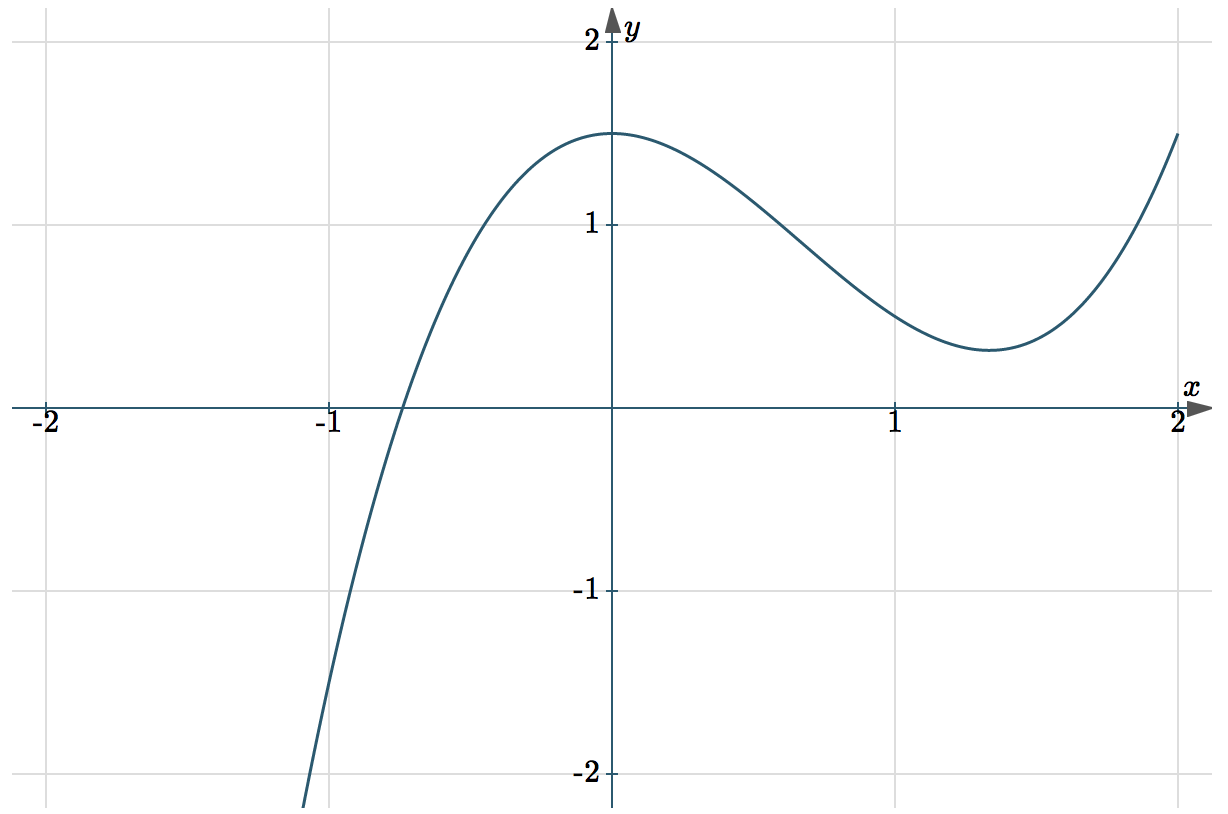
\includegraphics[width=0.25\textwidth]{../images/funplot.png}}\hfill
\fbox{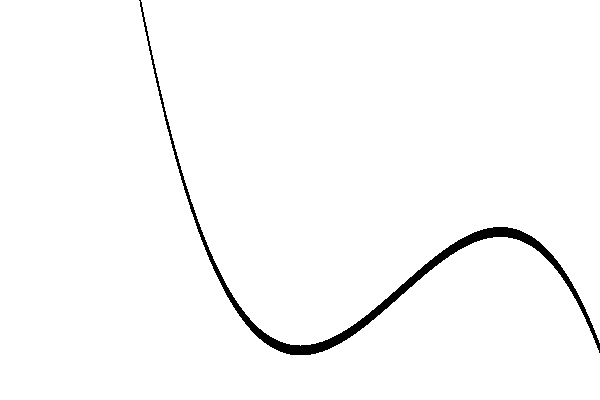
\includegraphics[width=0.25\textwidth]{../images/f.png}}\hfill
\fbox{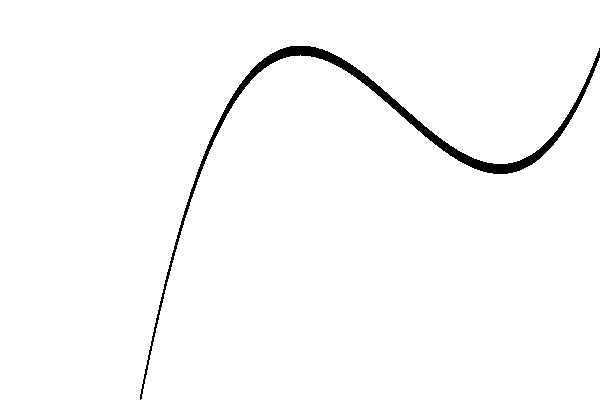
\includegraphics[width=0.25\textwidth]{../images/finv.png}}

\end{footnotesize}
\end{frame}

\begin{frame}[fragile]
\begin{footnotesize}

  \head{Tegning af Simple Relationer}

  \vspace{1ex}

  Vi kan også repræsentere en simpel relation som et funktionelt billede:

\begin{lstlisting}[numbers=none,frame=none,mathescape]
let circ : region =                        // $1 = x^2 + y^2$
  fun (x,y) -> 1.0 <<>> (x*x + y*y)
let coord : region =                       // +
  fun (x,y) -> x <<>> 0.0 || y <<>> 0.0
let (<||>) : region -> region -> region =  // combine regions
  fun r1 r2 -> fun p -> r1 p || r2 p
\end{lstlisting}

\head{Generering af PNG:}

\begin{lstlisting}[numbers=none,frame=none,mathescape]
do save600x400 "ccirc.png" (boolToFColor << (coord <||> circ))
\end{lstlisting}

  \vspace{1ex}

\fbox{
\includegraphics[width=0.25\textwidth]{../images/coord.png}}\hfill
\fbox{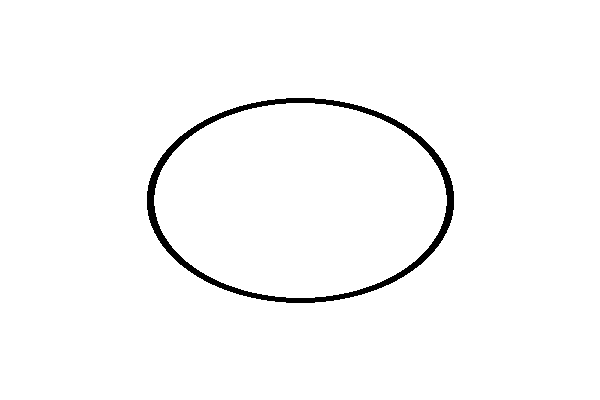
\includegraphics[width=0.25\textwidth]{../images/circ.png}}\hfill
\fbox{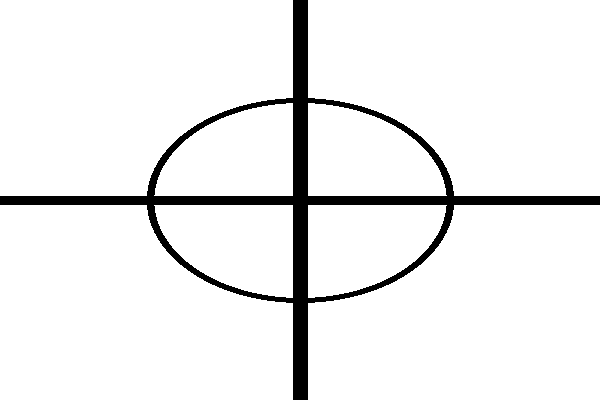
\includegraphics[width=0.25\textwidth]{../images/ccirc.png}}

\end{footnotesize}
\end{frame}

\begin{frame}[fragile]
\begin{footnotesize}

  \head{Skakbræt og Ringe}

  \vspace{2ex}

  Det er muligt at definere andre relationer såsom et skakbræt eller
  alternerende ringe:

\begin{lstlisting}[numbers=none,frame=none,mathescape]
let even x = x % 2 = 0
let floori x = int(floor x)
let checker : region =
  fun (x,y) -> even(floori x + floori y)

let distO (x,y) = sqrt(x*x+y*y)
let altRings : region =
  even << floori << distO
\end{lstlisting}

\mbox{ }\hfill
\fbox{
\includegraphics[width=0.25\textwidth]{../images/checker.png}}\hfill
\fbox{
\includegraphics[width=0.25\textwidth]{../images/altRings.png}}
\hfill \mbox{ }

\end{footnotesize}
\end{frame}

\begin{frame}[fragile]
\begin{footnotesize}

  \shead{Polære Koordinater}

  I det polære koordinatsystem bestemmes et punkt $p$ ved afstandet
  til centrum samt vinklen, i forhold til x-retningen, for linien der
  gennemgår centrum samt punktet.

  \sp

\begin{lstlisting}[numbers=none,frame=none,mathescape]
type polar_point = float * float
let toPolar ((x,y):point) : polar_point =
  (distO (x,y), atan2 y x)

let polarChecker n : region =
  let sc (r,t) = (r, t * float n / pi)
  in checker << sc << toPolar
\end{lstlisting}

\mbox{ }\hfill
\fbox{
\includegraphics[width=0.25\textwidth]{../images/polarChecker3.png}}\hfill
\fbox{
\includegraphics[width=0.25\textwidth]{../images/polarChecker5.png}}
\hfill \mbox{ }

\end{footnotesize}
\end{frame}

\begin{frame}[fragile]
\begin{footnotesize}

  \shead{Gråskalabilleder}
\begin{lstlisting}[numbers=none,frame=none,mathescape]
let wavDist : frac image =
  fun p -> (1.0 + cos (pi * distO p)) / 2.0

let save600x400s sz f img =
  toPngFile f (toCanvas sz img 600 400)

do save600x400s 7.0 "wavDist7.png" (fracToFColor << wavDist)
do save600x400s 9.0 "wavDist9.png" (fracToFColor << wavDist)
\end{lstlisting}

\mbox{ }\hfill
\fbox{
\includegraphics[width=0.25\textwidth]{../images/wavDist7.png}}\hfill
\fbox{
\includegraphics[width=0.25\textwidth]{../images/wavDist9.png}}
\hfill \mbox{ }

\end{footnotesize}
\end{frame}

\begin{frame}[fragile]
\begin{footnotesize}

  \head{Billedinterpolation og Farver}
  \sp

  To farver kan ``interpoleres'' med vægt \lstinline{w} $\in [0;1]$ som følger:

  \sp
\begin{lstlisting}[numbers=none,frame=none,mathescape]
let interpolC w (r1,g1,b1,a1) (r2,g2,b2,a2) : fcolor =
  let h x1 x2 = w * x1 + (1.0-w)*x2
  in (h r1 r2, h g1 g2, h b1 b2, h a1 a2)
let blueI : cimage = fun _ -> (1.0,0.0,0.0,1.0)
let redI  : cimage = fun _ -> (1.0,1.0,0.0,0.0)
\end{lstlisting}

\sp
Interpolation kan løftes til billeder:

\begin{lstlisting}[numbers=none,frame=none,mathescape]
let interpolI : frac image -> cimage -> cimage -> cimage =
  fun w a b p -> interpolC (w p) (a p) (b p)
let rbRings : cimage = interpolI wavDist redI blueI
let mystique : cimage =
  interpolI (fun _ -> 0.2) (boolToFColor<<checker) rbRings
\end{lstlisting}

\mbox{ }\hfill
\fbox{
\includegraphics[width=0.25\textwidth]{../images/rbRings.png}}\hfill
\fbox{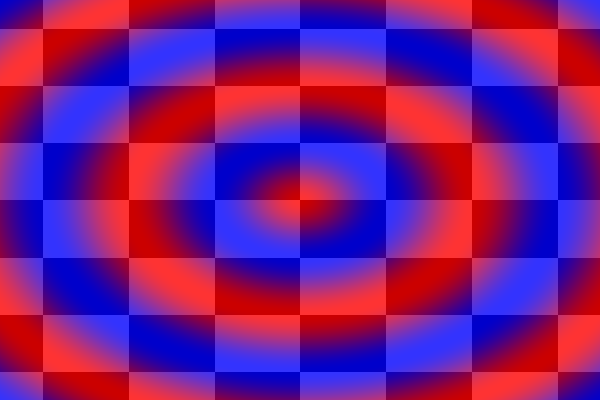
\includegraphics[width=0.25\textwidth]{../images/mystique.png}}
\hfill \mbox{ }

\end{footnotesize}
\end{frame}

\begin{frame}[fragile]
\begin{footnotesize}

\shead{Flere Muligheder}

Læs mere i
\begin{quote}
  Conal Elliott. Functional Images. Chapter in ``The Fun of
  Programming''. Book 2003. See
  \url{http://conal.net/papers/functional-images/}
\end{quote}

\sp \sp
Brug \lstinline{ImgUtil.runApp} til at styre parametre på
  køretid ved brug af tastaturinput.

  \sp

  \sp

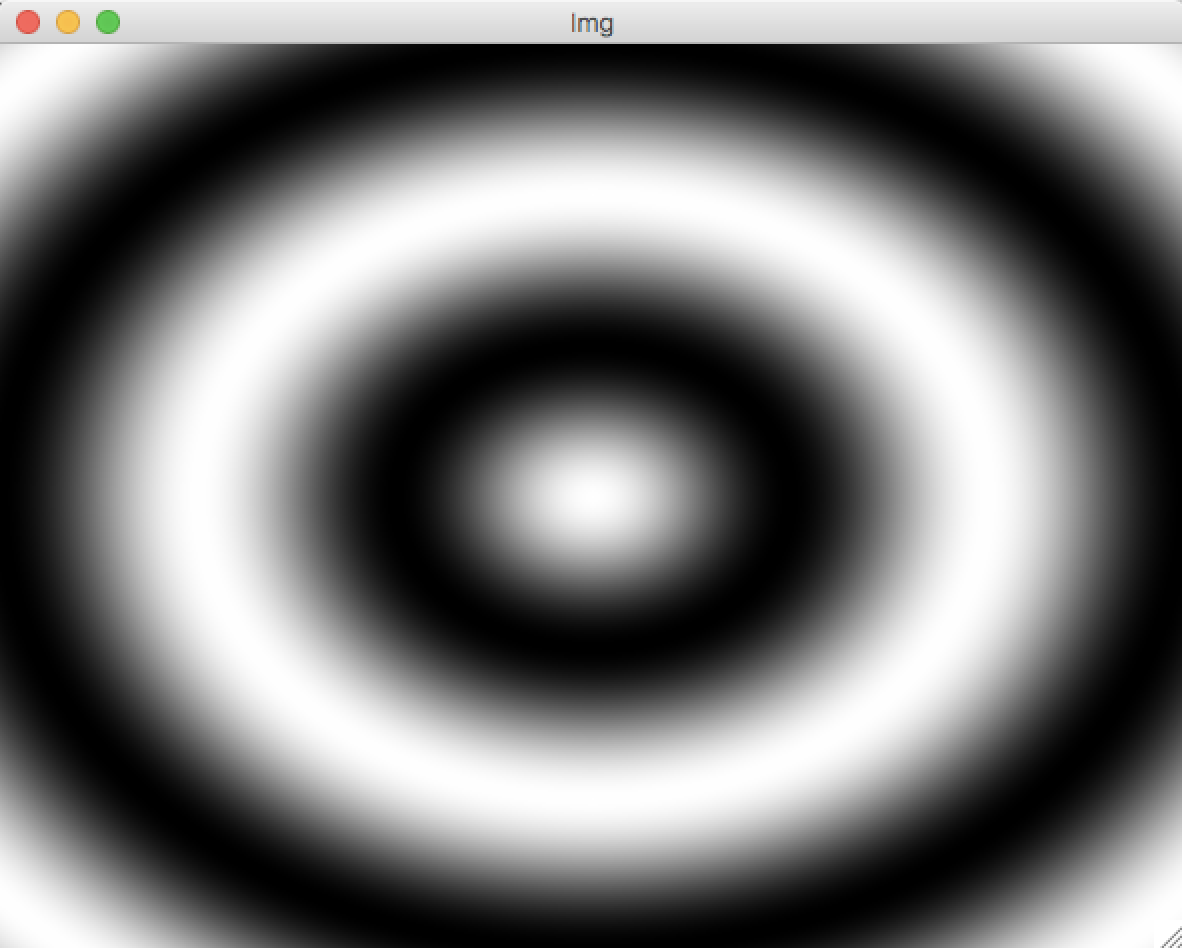
\includegraphics[width=0.30\textwidth]{../images/wav1.png}\hfill
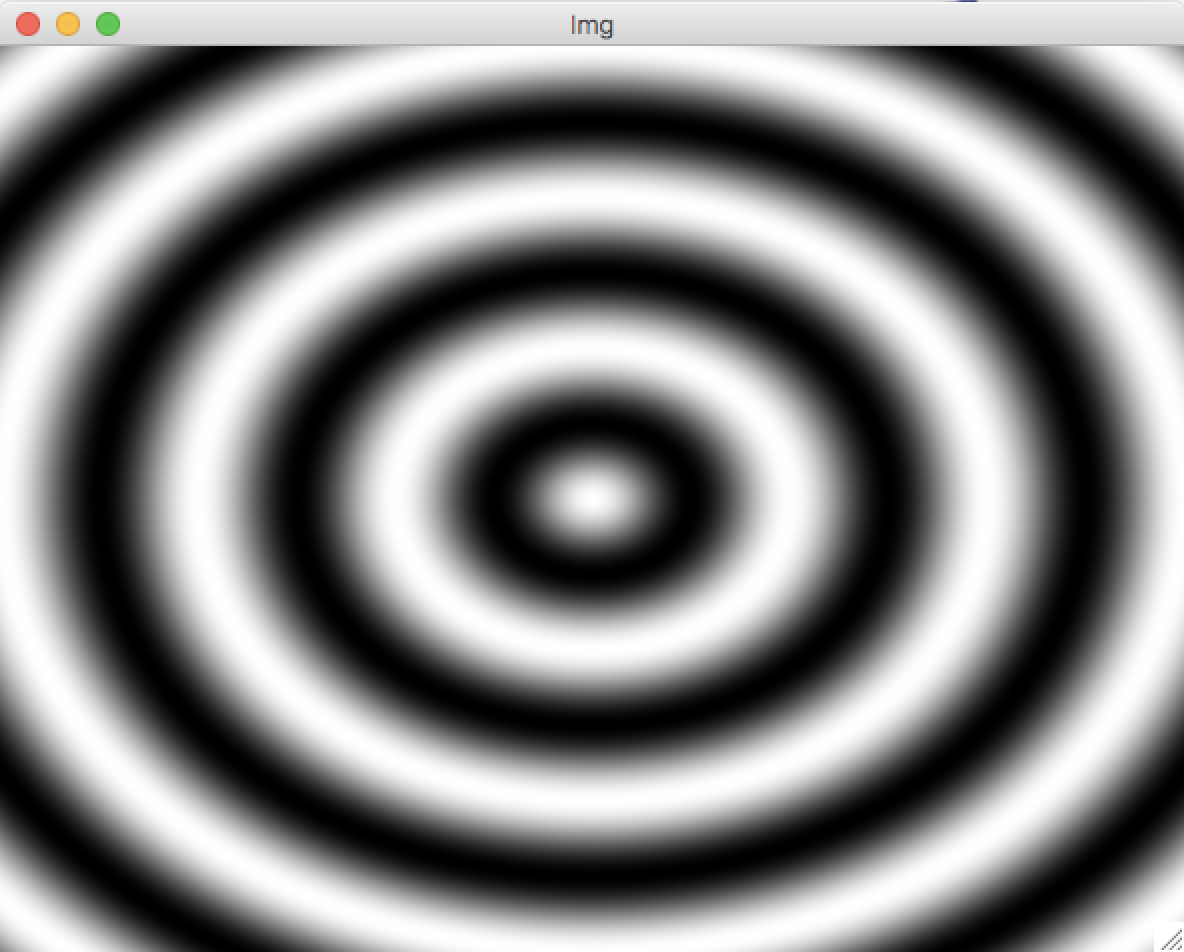
\includegraphics[width=0.30\textwidth]{../images/wav2.png}\hfill
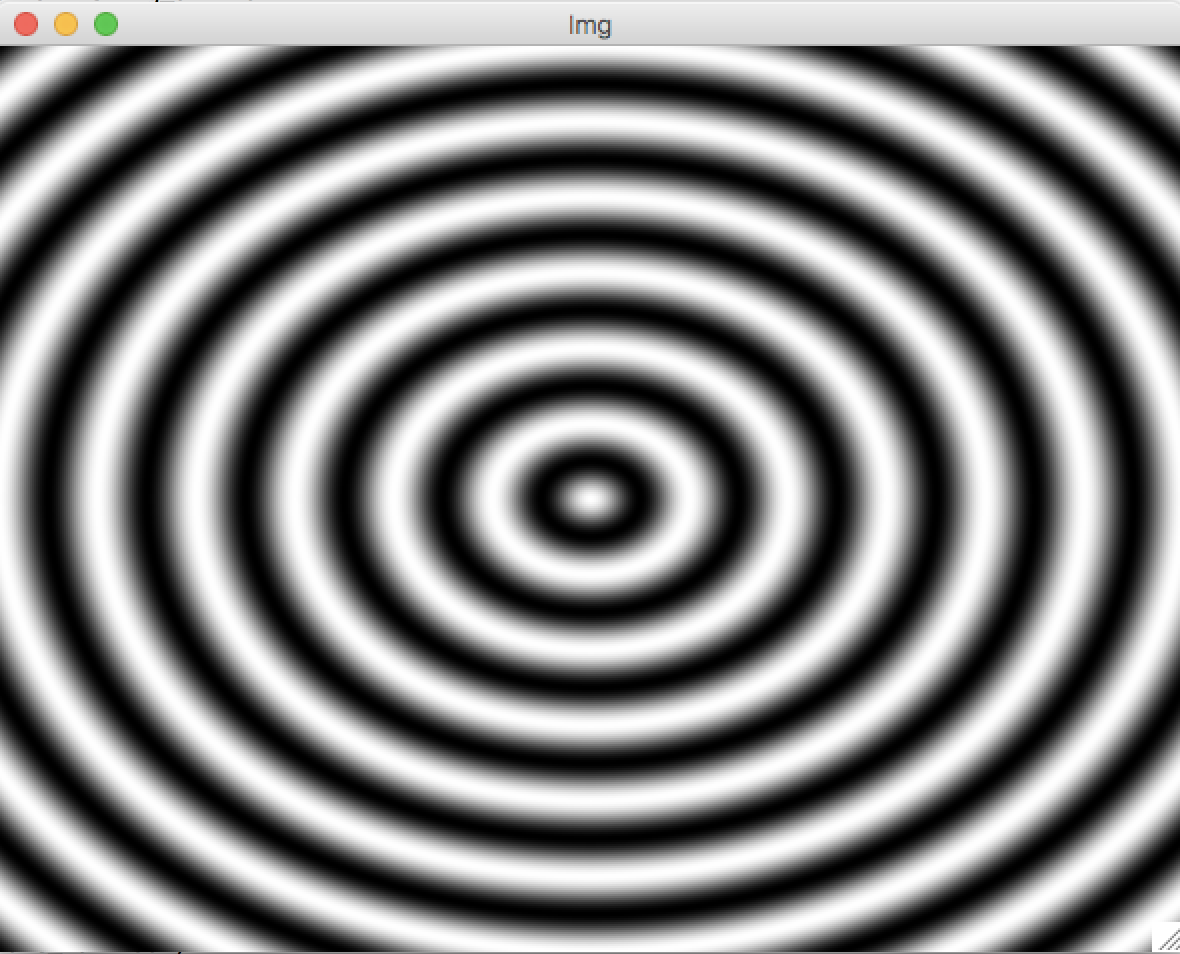
\includegraphics[width=0.30\textwidth]{../images/wav3.png}

\end{footnotesize}
\end{frame}

\subsection*{Konklusion}
\begin{frame}[fragile]
  \headsp{Konklusion}

  \vspace{3mm}
  \tableofcontents
\end{frame}

\end{document}
